\subsection{External Interface Requirements}
\subsubsection{User Interfaces}
The main way the users can interact with the system is via the mobile application for their smartphone, the interface should be user-friendly and in particular easy to read, with large and high contrast text to minimize reading problems in direct sunlight; the second way of connecting to the services provided is to use the web application their personal computer.
In both cases the user interfaces must satisfy the following constrains:
\begin{itemize}
	\item The first page must always ask the user to login or register to service.
	\item After the login, the system redirects the user to his/her home page.
	\item (Web) A toolbar must be present in every page, except login and registration page.
	\item (Mobile) A toolbar must be present in the homepage.
	\item The \emph{Create a meeting} page must provide a guided process to set-up a meeting and clearly show if the created meeting is not reachable in time from the location of a previous appointment.
	\item The \emph{Manage meetings} page must show a list of user's meetings divided by day and hour, and allows the user to select a meeting to obtain further information.
	\item The interface must offer the possibility to choose between a set of different languages.
	\item The user interface must dynamically adapt to the screen size.
	\item The Mobile and Web application must use the same graphical elements.
\end{itemize}
In addition to these constraints, other platform-dependent constraints are provided:
\begin{itemize}
	\item Web Application:\par
		All the pages must submit to W3C standards.
	\item Mobile Application:\par
		All mobile versions must follow the design guidelines provided by the respective platform manufacturer (Android, iOS, Windows \dots).
\end{itemize}
\subsubsection{Hardware Interfaces}
The web application needs any personal computer connected to the internet, while the mobile application must be able to connect to the network in order to exchange information with the server, such as destination and location of the user retrieved via the GPS of the mobile device.\\
Hardware requirements for both are later specified in \autoref{sec:HardwareLimitations}
\clearpage
\subsubsection{Software Interfaces}
\label{sec:SoftwareInterfaces}
Supported browsers for the web application should include Google Chrome, Mozilla Firefox, Opera, Safari, Internet Explorer and Edge, while the mobile application must be available on Android, iOS, Windows Phone and Blackberry OS.\\
The server side of the application requires: 
\begin{itemize}
	\item \href{http://www.oracle.com/technetwork/java/javaee/overview/index.html}{Java EE}, to write the server application that perform the travel computation and the database access.
	\item \href{https://dev.mysql.com/}{MySQL}, to memorize user information and meetings inside a relational database.
\end{itemize}
The client side of the application requires the latest version of the platform SDK.
\subsubsection{Communication Interfaces}
The client communicates to the server via HTTPS protocol using TCP.\\
In addition, the system must be able to use the API of other application in order to retrieves weather and news about road conditions or strike.

\clearpage

\subsection{Functional Requirements}

\subsubsection{Registration}

\paragraph*{Purpose\\}

The main purpose of the \emph{Registration} use case is to provide the user a service which permits the subscription to the system. The user must fill a registration form with his/her personal information and accept the Terms and Conditions of use. After that a confirmation e-mail is sent to the specified e-mail.

\paragraph{Functional Requirements}
\begin{enumerate}[label=R.\arabic*:]
	\item The system must not accept an already registered e-mail.
	\item The user must provide the following information:
	\begin{itemize}
		\item name
		\item surname
		\item e-mail
		\item password
	\end{itemize}
	\item The system cannot allow the user to proceed in the registration process if he/she does not accept the Terms and Conditions of use.
	\item The system must send an e-mail to the user after he/she submits the form.	
	\item The system must generate a unique link for the registration e-mail.
	\item The user must be able to exit the form any time.
\end{enumerate}

\paragraph*{Use Case\\}
The use case of \emph{Registration} is analysed in Table \ref{tab:registration}.

\begin{longtable}{p{0.25\linewidth}p{0.75\linewidth}}
	\hline
	\textbf{Name} & \textbf{Registration} \\
	\hline
	\textbf{Actors} & Non registered user \\
	\hline
	\textbf{Entry conditions} & \_ \\
	\hline
	\textbf{Flow of events} & 
	\begin{enumerate}
		\item The user asks to the system to register to its service.
		\item The system shows the appropriate form to fill.
		\item The user fills the form inserting its own information.
		\item The user submits the form.
		\item The system checks if the e-mail is unique.
		\item The system sends to the specified e-mail address a confirmation e-mail with a unique link.
		\item The user must open the e-mail and click on the confirmation link.
		\item The system receives the confirmation, saves the data inside a database and notifies to the user.
	\end{enumerate}\\
	\hline
	\textbf{Exit conditions} & The user is now registered and he/she can login and start to use the service.\\
	\hline
	\textbf{Exceptions} & Exceptions can occur when requirements R.1, R.2 and R.3 are violated, in this case the system reloads the registration form and goes back to step 2. 
	Registration process is also aborted when the user decides to complete it. \\
	\hline
	\caption{\emph{Registration} use case description}
	\label{tab:registration}
\end{longtable}

\paragraph*{Activity Diagram\\}
The activity diagram of \emph{Registration} use case in showed in Figure \ref{fig:registrationac}

\begin{figure}[h]
	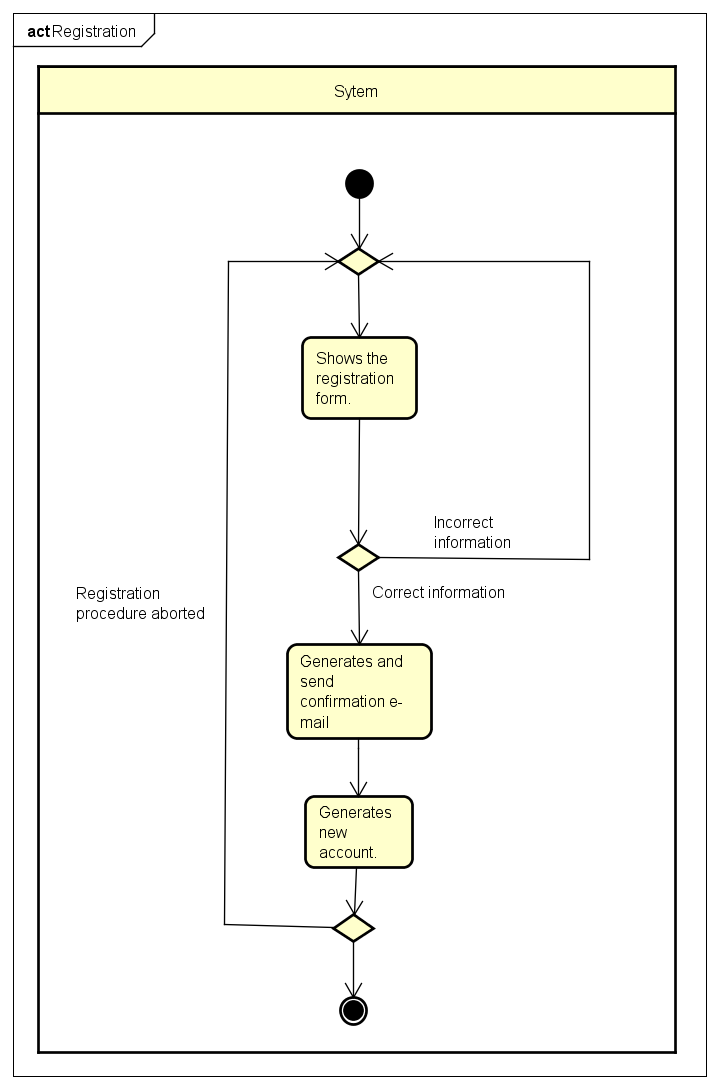
\includegraphics[width=\textwidth,height=\textheight]{Img/RegistrationAC}
	\caption{\emph{Registration} activity diagram}
	\label{fig:registrationac}
\end{figure}

\begin{figure}
	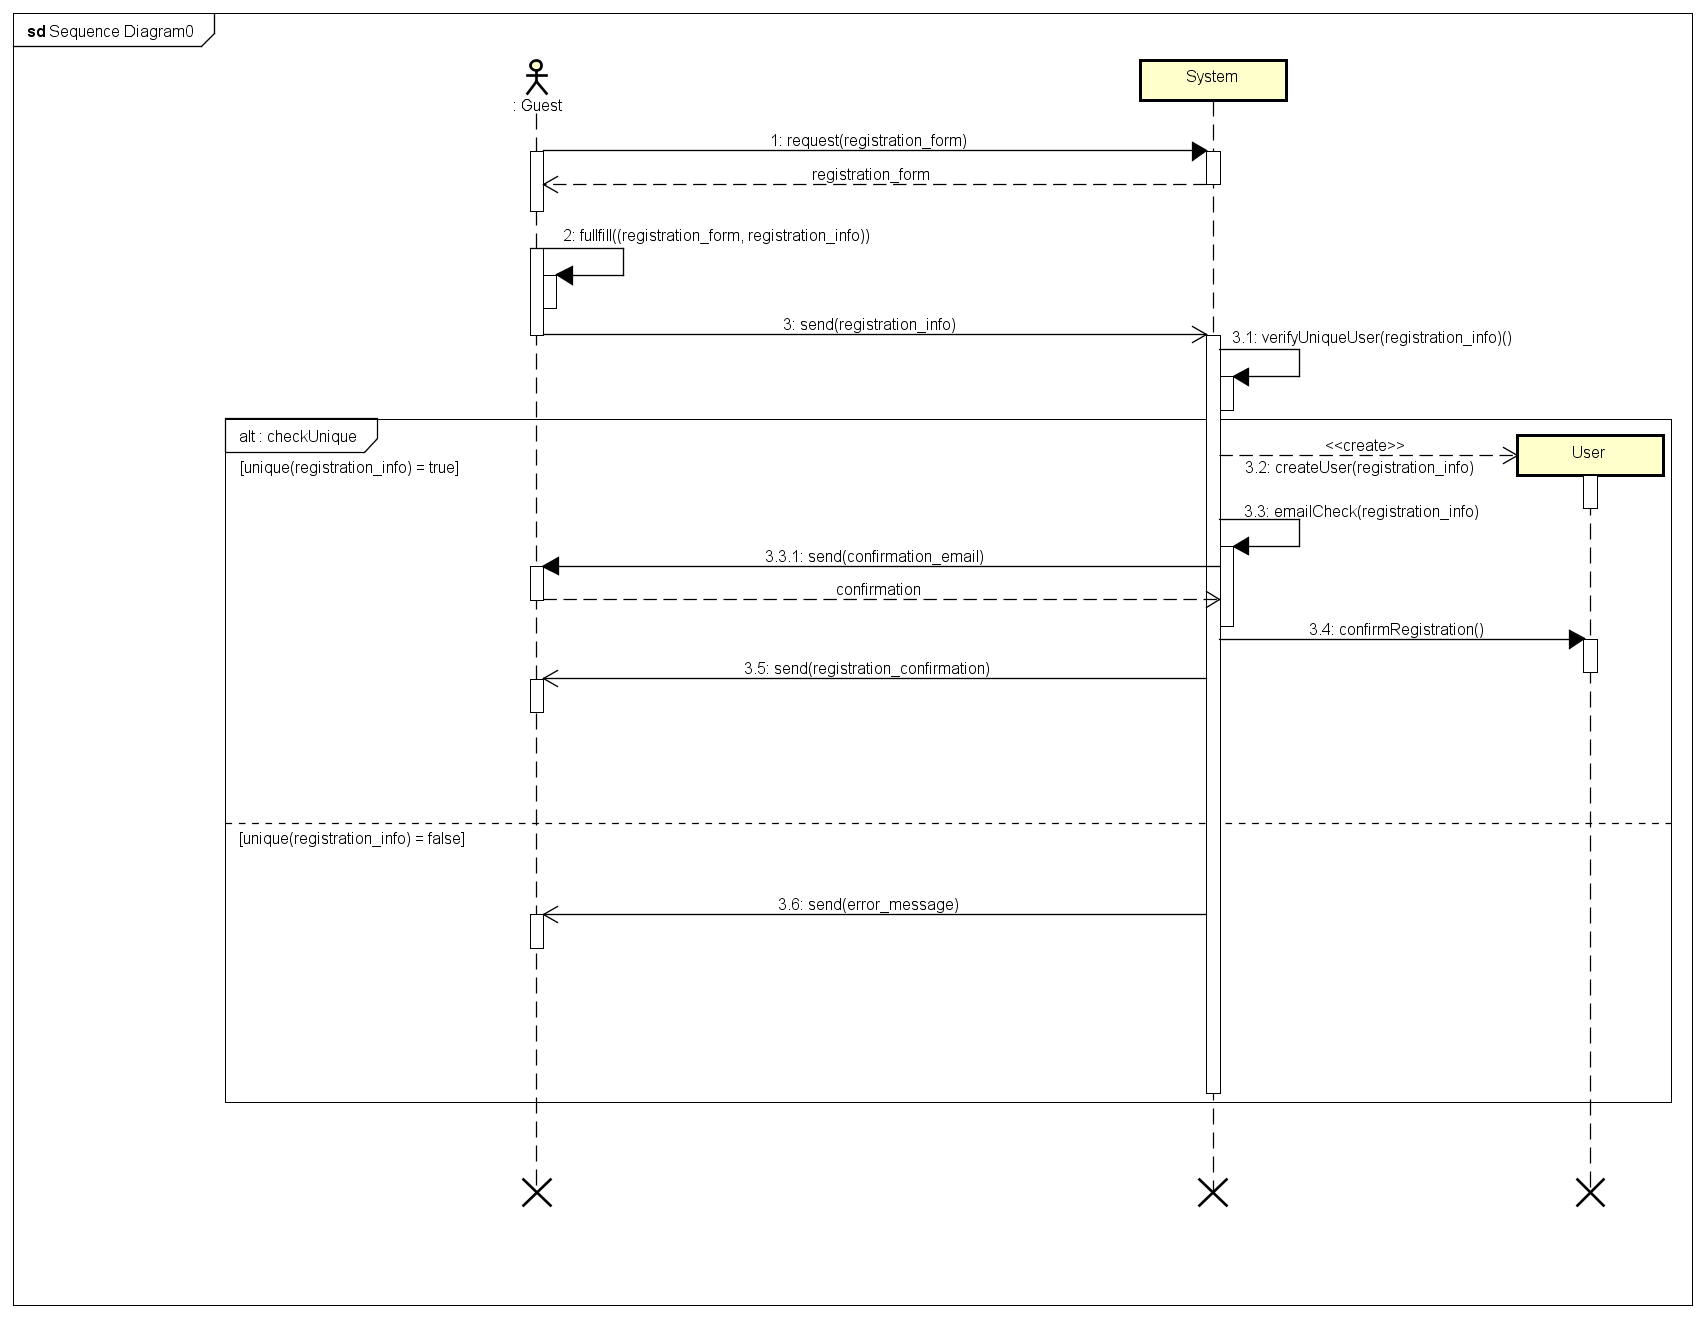
\includegraphics[width=\textheight,height=\textwidth,angle=90]{Img/RegistrationSQ}
	\caption{\emph{Registration} sequence diagram}
	\label{fig:registrationsq}
\end{figure}


%Add Use cases----------------------------------------------------
\clearpage
\subsection{Performance Requirements}
Without taking into consideration the speed of the internet connection, in order to guarantee an acceptable user experience the following  requirements must be satisfied:
\begin{itemize}
\item Navigation between pages of the system must happen in 0.5s or less.
\item The  best travel plan must be computed in 5s or less.
\item No limit of registered users in the database.
\item No limit of schedulable appointments.
\item At least 1000 users must be able to use the service at the same time. 
\end{itemize}
\newpage
\subsection{Design Constraints}
\subsubsection{Standards Compliance}
The web application must comply with the standards dictated by W3C, while the mobile application must follow the Oracle guidelines for Java programming.
\subsubsection{Hardware Limitations}
\label{sec:HardwareLimitations}
Minimum system requirements for the two applications:
\begin{itemize}
\item Web application
\begin{itemize}
\item 512Mb of RAM.
\item 2Mb/s internet connections.
\item 800X600 screen resolution.
\end{itemize}
\item Mobile application
\begin{itemize}
\item 1Gb of RAM.
\item 3G UMTS internet connections.
\item 100Mb of free space.
\end{itemize}
\end{itemize}
The system should also be able to process operations in parallel.
\clearpage
\subsection{Software System Attributes}
\subsubsection{Reliability}
Each trip plan computed given the preferences expressed by the user and the weather forecast and strikes must not differ more than 5\% from the optimal travel distance or ETA.
\subsubsection{Availability}
The system to be must guarantee an availability of no less than 98\%.
\subsubsection{Safety and Privacy Constraints}
The user oversees his/her own security while travelling and must grant access to the current location, information about former trips and personal data are stored but only the user itself has access to them.
\subsubsection{Maintainability}
The system must be developed in such a way that future implementation of new features and changes to existing ones can be done seamlessly, in other words the system has to be modular and scalable.
\subsubsection{Portability}
As already mentioned in \autoref{sec:SoftwareInterfaces} the software must be available on different configurations, it must be as environment independent as possible, meaning that it has to work on different platforms with the minimum amount of changes to the software itself.


